\chapter{体型异常}

体型是身体各部分,包括骨骼、肌肉的成长与脂肪分布等发育状态的外观表现。体型异常则是指一个人的体型与同种族、同年龄、同性别的参考人群比较存在显著差异(通常超过2个标准差),包括矮小体型、高大体型、肥胖及消瘦四大类,常伴有青春期启动及第二性征发育的异常而引起重视。

一个人体型的高矮主要取决于骨骼的发育,即骨骼纵向拉伸的程度及骨骼成熟、骨骺闭合的时间。影响骨骼发育的内分泌激素最重要的是生长激素、性激素及甲状腺素。生长激素是重要的生长调节因子,能促进骨骼、软骨、肌肉及其他组织的细胞分裂、增殖和蛋白质合成,同时促进钙、磷的摄取和利用,增加骨骼纵向拉伸所需的原料。生长激素促进骨骼发育的作用是通过胰岛素样生长因子-1(IGF-1)所介导的。胎儿期机体对生长激素极不敏感,如孕12周胎儿体内已可检测到血生长激素浓度,至孕20周时生长激素分泌达最高峰(100~150μg/L),出生后机体迅速恢复对生长激素的敏感性,在远低于胎儿期生长激素浓度的刺激下出现人体生长发育的第一个高峰。出生后第一年身材增长最快,前3个月每月增高3.0~3.5cm,第3~6个月每月增长2.0cm,第6~12个月每月增长1.0~1.5cm,因此出生后第1年累积身材增长约25cm。1~2岁全年约增高10cm,此后平均每年增高约5~8cm。因此,若存在生长激素缺乏,细心的家长往往在小儿2~3岁甚至更早即可发现孩子身材增长落后于同龄儿童。同理,若生长激素分泌过多,也可较早被发现,且每年身高增长的幅度也显著高于同龄儿童。人体生长发育的第二个高峰出现在青春期启动后,中枢抑制解除后,性激素大量分泌,性激素对骨骼发育的影响,在青春期早中期主要促进骨骼的纵向拉伸,与生长激素协同作用导致身材激增,在青春期晚期则促进骨骺闭合,骨骼纵向拉伸停止。青春期平均启动年龄为10~12岁,女孩比男孩早1~2年,身材激增持续3年左右,男孩可每年增长7~9cm,女孩每年增长6~8cm,整个青春期男孩平均增长约28cm,女孩增长约25cm。青春期启动过早(性早熟),患儿青春早中期身材明显高于同龄儿,但由于骨骺提前闭合,最终身高将落后于同龄人。相反,若青春期延迟启动或性激素分泌不足,则青春期身材激增不明显而身高落后于同龄儿,且伴第二性征发育不良,但由于骨骺闭合延迟,性成熟年龄过后(成年期)骨骼纵向拉伸仍未停止,最终累积身高并不落后,甚至可高于正常人群。甲状腺素对骨骼发育的作用主要是刺激软骨生长,促进骨的生长与成熟,使骨骼发育保持合适比例。由于甲状腺素缺乏而导致矮小体型者通常幼年起病,神经系统发育也因甲状腺素不足而受累,患儿除身材矮小外,常伴智力缺陷及特殊面容,旧称“呆小病”。此外,遗传因素、营养状况、环境、社会心理、全身性疾病等均可影响生长发育。

体型的胖瘦主要取决于体内脂肪含量的多少,后者是能量摄入与消耗之间平衡的结果,与机体的营养状况密切相关,除家族遗传因素外,常与多种内分泌代谢性疾病有关。下丘脑是人体食欲、睡眠、行为中枢,下丘脑功能紊乱常导致患者贪食或厌食、嗜睡或失眠,从而引起患者肥胖或消瘦。垂体是多种内分泌轴的上游中枢器官,分泌多种促激素调节下游靶腺功能,参与能量的摄入与消耗。垂体或靶腺功能异常引起的继发性或原发性靶腺功能亢进或减退,可导致机体肥胖或消瘦。譬如甲状腺功能亢进症引起机体代谢率升高、能量消耗增多而致消瘦,甲状腺功能减退症降低代谢水平及能量消耗而致肥胖。皮质醇增多症致水钠潴留、脂肪向心性积聚而增加体重,肾上腺皮质功能不全则往往致体液丢失而使体重下降。此外,胰岛素、儿茶酚胺、生长激素等均影响能量代谢及脂肪的合成与分解。

体型异常是指某人的体格发育与同一种族、年龄、性别正常人的身长、体重及形态有显著差异者,譬如体型过高、过矮、过胖、过瘦及其他形态异常等。体型异常显而易见,常能作为引导诊断的重要线索。

\section{【引起体型异常的因素】}

主要有下列几方面:

\subsection{(一)先天性因素}

遗传及体质因素对生长发育以及由此形成的体格起一定的作用。母体在妊娠期间患病或营养不足以及早产等,也可引起先天性生长发育异常。

\subsection{(二)营养及代谢障碍}

营养缺乏如缺碘(地方性呆小症)、维生素D缺乏(佝偻病);全身慢性疾病可影响生长发育而致侏儒;脂质代谢障碍等可引起肥胖;高度营养不良可引起消瘦。

\subsection{(三)内分泌功能障碍}

生长激素、甲状腺素、胰岛素及性激素与生长发育有密切关系。例如生长激素过多则引起巨人症或肢端肥大症,生长激素过少可引起垂体功能减退性侏儒症;甲状腺素过少引起呆小症;Klinefilter综合征性激素过少,使骨骺融合延迟而形成过高体型,而Turner综合征卵巢发育不良则以身材矮小为主要特征。此外,肾上腺皮质激素过多可引起肥胖,过少则可引起消瘦。

\subsection{(四)神经系统功能障碍}

中枢神经系统疾病如脑炎、脑膜炎、结核、梅毒、肿瘤等,可由于下丘脑受累而引起生长发育异常、肥胖或消瘦。

本章主要讨论下述四种体型异常:①高大体型;②矮小体型;③肥胖;④消瘦。引起各种体型异常的疾病很多(表\ref{tab40-1}),分节顺序讨论于下。

\begin{longtable}{c}
 \caption{高大体型、矮小体型、肥胖与消瘦的疾病分类}
 \label{tab40-1}
 \endfirsthead
 \caption[]{高大体型、矮小体型、肥胖与消瘦的疾病分类}
 \endhead
 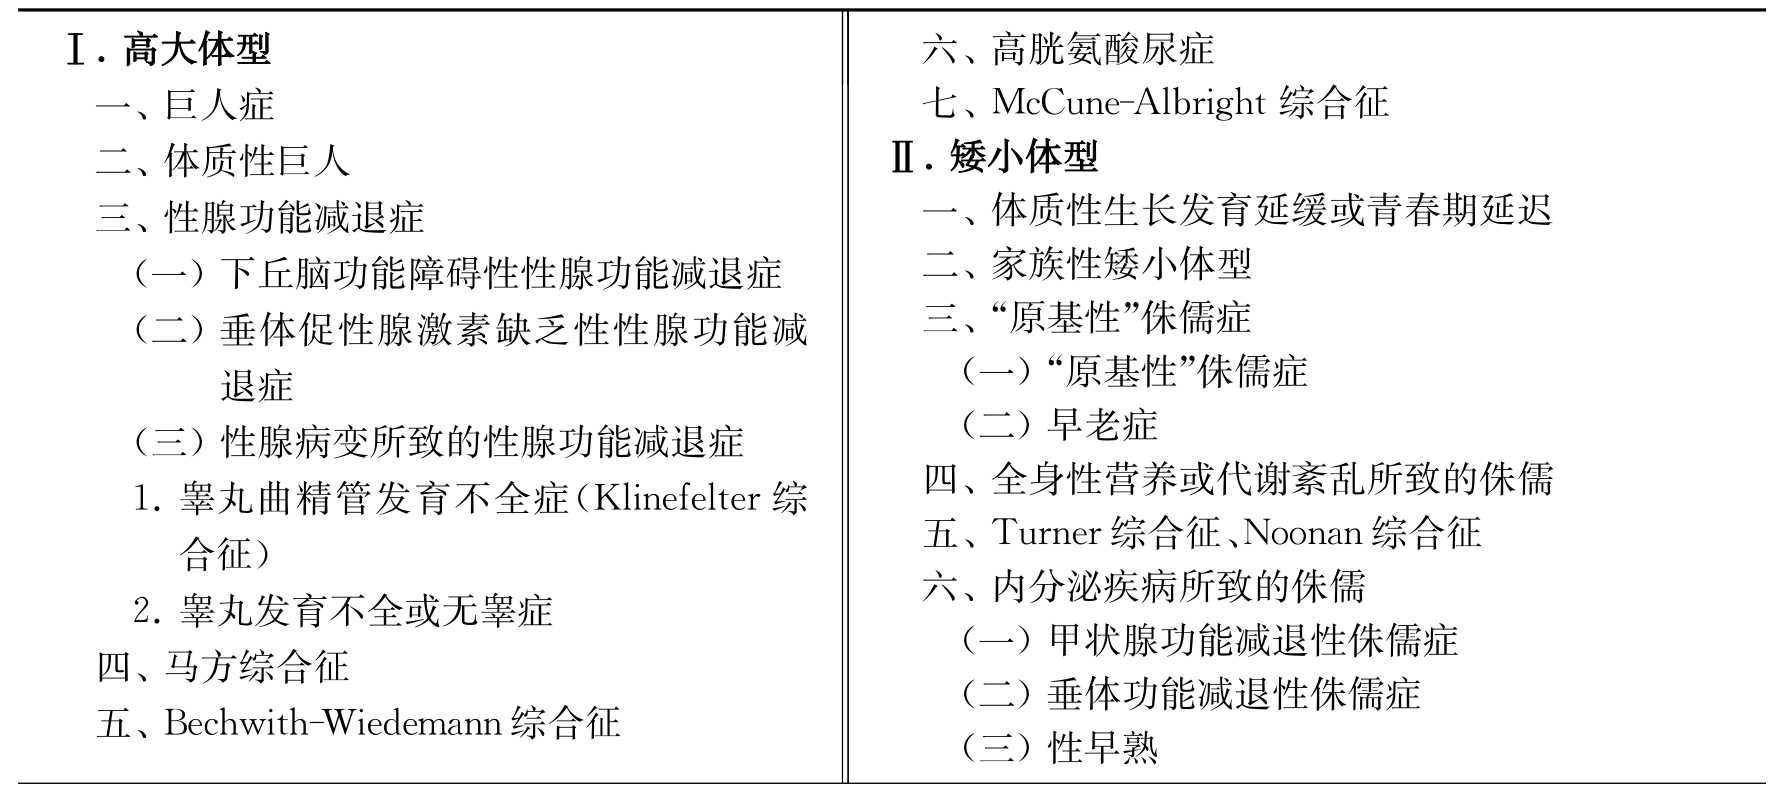
\includegraphics[width=\textwidth,height=\textheight,keepaspectratio]{./images/Image00247.jpg}\\
 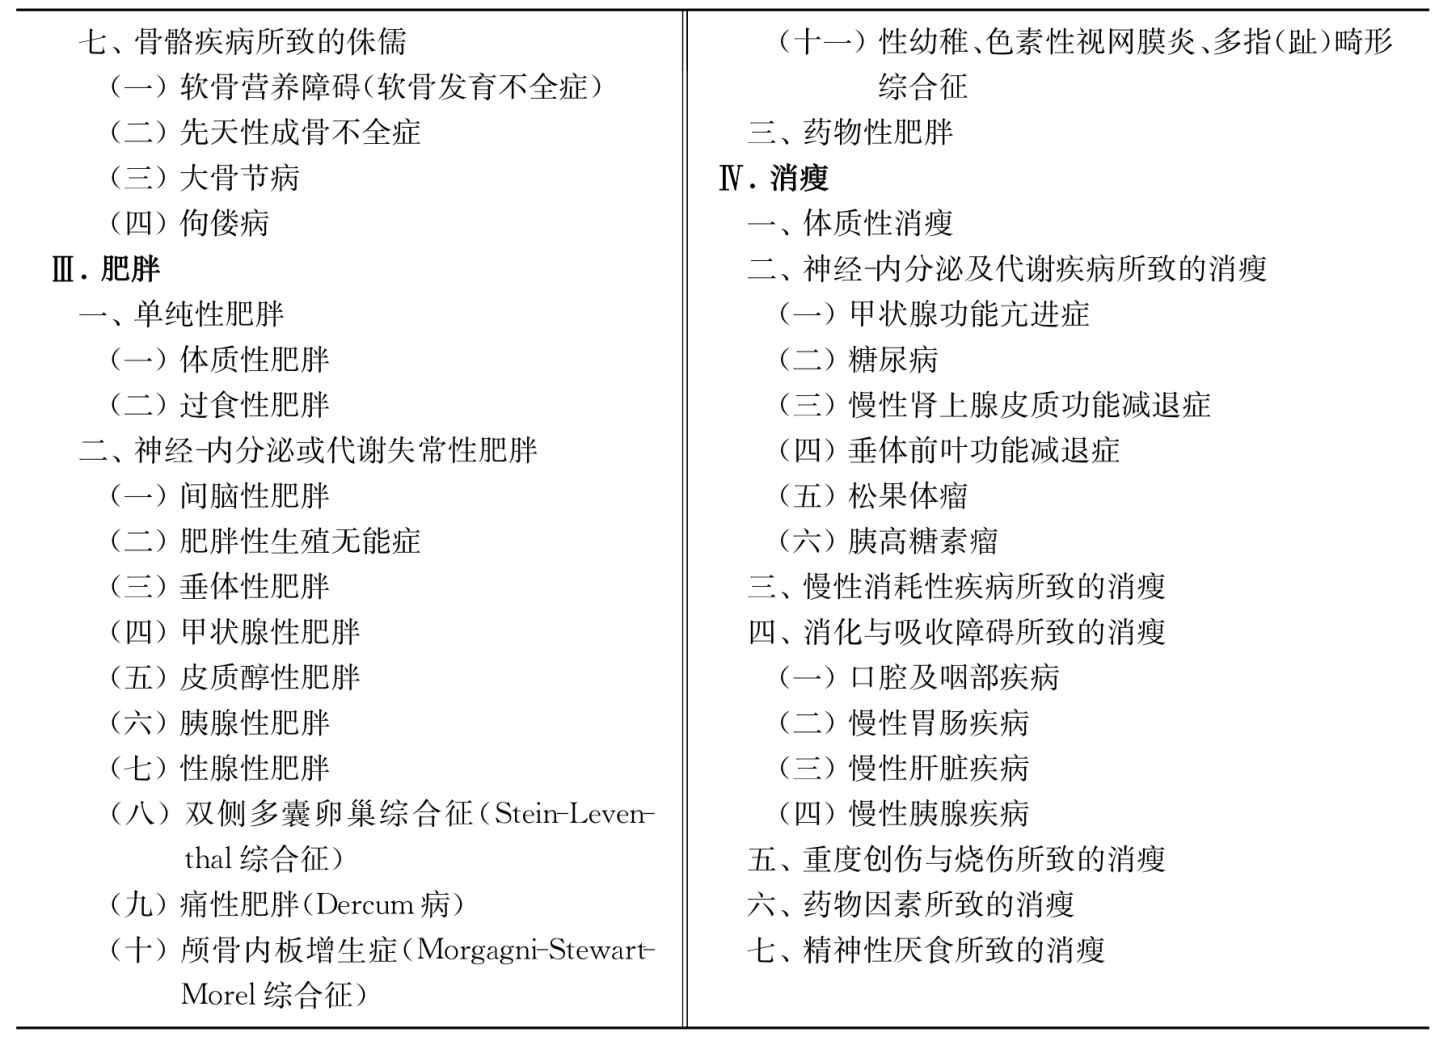
\includegraphics[width=\textwidth,height=\textheight,keepaspectratio]{./images/Image00248.jpg}
 \end{longtable}

\protect\hypertarget{text00312.html}{}{}

\section{132 高大体型}

高大体型并无通用标准,也缺乏流行病学资料,一般认为身高超过同种族、同年龄、同性别参考人群的身高标准即为高大体型。据此定义,高大体型并不特指受检者的最终身高,可包括生长发育某一个时期与同龄人比较的结果,譬如性早熟患儿,由于青春期提前启动,在青春期的早中期身材激增,可明显高于同龄儿,呈现高大体型,但由于性激素促使骨骺提前闭合,患者成年身高反而矮于同龄正常人。因性早熟在前述矮小体型中已作为病因分类之一,故不在此参与高大体型的病因构成。高大体型的发生与遗传及内分泌因素关系密切,除身材高大外,由于相应激素分泌异常或合并肿瘤等,可出现多种并发症而导致器官功能损害,因此,以高大体型为线索,寻找内分泌功能异常,对因处理,将有利于减少并发症,延缓器官功能衰退。

对于高大体型患者病史询问应包括出生时身长、体重、生母妊娠分娩情况,出生后喂养情况、饮食运动睡眠习惯,何时开始出现身材增长快于同龄人,身材增长的速度(cm/年),青春期启动时间,第二性征发育情况(如晨勃、遗精、月经初潮等),家族中有无类似病患,父母及同胞的体型,有无合并头痛、视力下降、视野缺损,有无合并尿崩症表现,有无嗅觉障碍等。体格检查方面,应测量身高、体重、上、下部量、两指间距、喉结、胡须、腋毛、阴毛、乳房、外生殖器发育情况、嗅觉、有无特殊面容等。

高大体型者需考虑以下疾病:

\subsection{一、巨人症}

一般认为男性身高>2.0m,女性身高>1.85m即为巨人症,但需注意人种差异。巨人症与肢端肥大症一样,均由垂体肿瘤分泌过多生长激素引起,前者起病于幼年骨骺闭合前,以高大体型为突出表现,后者则发病于成年期、骨骺闭合后,身材多正常,而以骨膜增厚、器官肥大、特殊面容为主要表现。巨人症最常见的病因为垂体生长激素肿瘤或生长激素/泌乳素混合瘤,多数肿瘤生长缓慢,部分患者可表现为病情活动一段时间后进入非活动期。

过度分泌的生长激素促进长骨纵向生长加速,身材明显高于同龄儿童,并且持续加速增长,至青春期结束后通常达到1.85m(女性)及2.0m(男性)以上。进入成年期后,若病因未处理,生长激素持续过多分泌则可导致面部、手足等部位软组织增厚增粗,面容改变如颧骨及下颌骨增大突出、眉弓外突、牙齿错位、咬合不良,鼻部、舌头增厚肥大,声带厚长,声音低沉。内脏器官增大肥厚,血管壁及呼吸道黏膜增厚,可并发高血压、高动力型肥厚型心肌病、冠状动脉硬化性心脏病、呼吸道阻塞、通气阻力增大、呼吸功能障碍等。生长激素拮抗胰岛素作用,故巨人症患者常合并糖耐量减低或糖尿病。由于生长激素具有促增殖作用,患者肿瘤发生风险明显增加,其中以结肠息肉、胃肠肿瘤及腺癌与生长激素分泌过多关系尤为密切。

垂体生长激素肿瘤一般以大腺瘤(直径>1.0cm)或巨腺瘤(直径>3.0cm)多见,故常出现肿瘤压迫表现,包括头痛、视野缺损、视神经萎缩、动眼神经麻痹、下丘脑功能障碍等。肿瘤压迫正常垂体组织,久病可出现垂体前叶功能减退表现,首先性腺轴受累,随后甲状腺及肾上腺皮质功能减退,患者出现相应垂体前叶功能减退症状。部分患者垂体生长激素大腺瘤生长迅速,可发生肿瘤出血、梗死或坏死,出现垂体卒中,表现为剧烈头痛、呕吐、视野缺损,若瘤内容物或出血进入蛛网膜下腔,可引起发热、颈项强直等脑膜刺激征,甚至出现昏迷。

根据患者突出的高大体型,巨人症一般很难漏诊,诊断的关键是内脏器官受累情况的评估及病因的寻找。生长激素分泌过多的证据主要是血清生长激素、IGF-1及IGF-BP3显著升高,后两者需结合患者年龄与同年龄、同性别参考人群进行比较。口服葡萄糖耐量试验仍为目前临床最常用的确诊手段,于服糖前30分钟及服糖后30、60、90、120分钟分别采血测生长激素,正常人服糖120分钟后,生长激素降至2μg/L或更低。巨人症患者服糖后生长激素不被抑制,或部分抑制未达正常人水平。垂体其他促激素及靶腺激素水平也应进行常规评估。

影像学检查可做垂体CT或MRI明确肿瘤部位。确立巨人症诊断时还需要考虑以下几点:①明确是单一生长激素肿瘤还是生长激素/泌乳素混合瘤,或其他导致生长激素分泌过多的病变(如生长激素释放激素分泌异常);②判断生长激素瘤的良恶性以及肿瘤的侵袭性;③是否存在垂体前叶功能减退症,有无继发性糖尿病、视力障碍、肿瘤等并发症;④排除多发性内分泌腺瘤综合征(MEN-I)和G蛋白病(McCune-Albright综合征)的可能。

\subsection{二、体质性巨人}

体质性巨人可能与遗传有关,父母及同胞或近亲也有高大体型表现。引起生长过度和身材过高的原因与生长激素无关,其特点为身高虽远超于正常人,但身体各部分生长发育匀称,体力好,生育能力正常,不伴内分泌功能障碍,也无特殊的并发症及代谢异常,身体各方面检查均正常,属正常身高变异而非病态。体质性巨人与垂体生长激素肿瘤引起的巨人症在身高方面可无明显的分界。

\subsection{三、性腺功能减退症}

先天性下丘脑或垂体发育不良或遗传性染色体病等所致继发性或原发性性腺功能减退症,常于幼年起病,尤其不伴生长激素分泌缺陷者,骨骼过度生长,骨骺不闭合,故患者体型高大,四肢细长,与躯干不成比例,下部量长于上部量,两指间距长于身高,形成瘦高身材,第二性征缺如,性腺发育不良。

根据发病部位,性腺功能减退症引起的高大体型可分为以下三种病因:

\subsubsection{(一)下丘脑功能障碍性性腺功能减退症}

由于下丘脑病变如颅咽管瘤、神经胶质瘤、炎症等引起,幼年发病可致高大体型,常伴下丘脑功能紊乱表现,如尿崩症、情绪改变、睡眠障碍、体温调节异常、食欲改变、肥胖或消瘦等。

\subsubsection{(二)垂体低促性腺激素性性腺功能减退症}

垂体病变若仅累及性腺轴,则患者常为高大细长体型,实验室检查显示FSH,LH及性激素显著降低,不被GnRH兴奋,且无其他垂体激素分泌不足表现,若合并嗅觉障碍,需注意Kallman综合征诊断。

\subsubsection{(三)性腺病变所致原发性性腺功能减退症}

最典型的是男性起病的Klinefelter综合征,属于染色体病,染色体核型为47,XXY或包含47,XXY的各种嵌合体核型。此外,睾丸发育不全或无睾症、由于幼年疾病(炎症、放射损伤、外伤等)所致睾丸损伤、睾丸发育不良均可致原发性性腺功能减退症,实验室检查提示雄激素降低,LH、FSH显著升高。

\subsection{四、马方综合征}

属于常染色体显性遗传性结缔组织病,为先天性中胚层发育不良所致,临床罕见,常有家族史。病变主要累及骨骼、眼和心血管系统,智力多不受影响。患者表现为高大体型,四肢尤其手指脚趾细长,呈蜘蛛足样改变,皮下脂肪少,胸廓发育外凸畸形或狭长如鸡胸,常有高度近视、晶状体脱位等眼部表现,先天性心血管畸形常见为主动脉瓣关闭不全、主动脉动脉瘤、二尖瓣关闭不全等。

\subsection{五、Bechwith-Wiedemann综合征}

又名脐疝-巨舌-巨体综合征,或新生儿低血糖-巨舌-内脏肥大-脐膨出综合征,是一种罕见的遗传病,病因不明。该病多呈散发性,也有家族性发病的报道,为常染色体隐性遗传,或常染色体显性遗传外显不全。临床特点是:高大体型、巨舌、脐膨出或脐疝、高胰岛素性低血糖症,一侧性身体不对称性肥大,内脏肥大、并伴有心血管损伤,如心肌肥厚、先天性心血管畸形,10\%患者可伴胚胎性肿瘤。生长激素分泌正常。

\subsection{六、高胱氨酸尿症}

为常染色体隐性遗传病,临床表现为身材瘦长、四肢细长、两颧潮红、毛发纤细稀疏、韧带松弛、智力发育迟滞。存活患者眼、骨骼与血管病变类似马方综合征,尿中高胱氨酸可用氰化硝普盐试验检测以明确诊断。

\subsection{七、McCune-Albright综合征}

又称多发性骨纤维发育不良症,临床以骨骼损害、性早熟和皮肤色素沉着为主要表现,少数患者可合并其他内分泌功能异常。青春期提前启动及伴发生长激素分泌过多,使患儿体型较同龄儿明显高大。

本病诊断的主要依据:①具有骨损害、皮肤色素沉着和性早熟3大主要临床表现;②具有骨纤维结构不良的X线表现,皮肤Cafe-au-lait斑;③年龄在30岁以下年轻患者,伴有内分泌或非内分泌异常表现;④GNAS1基因突变。

\protect\hypertarget{text00313.html}{}{}

\section{133 矮小体型}

矮小体型,又称身材矮小症,指与同地区、同年龄、同性别参考人群比较,身高低于平均身高的2个标准差(2s)以上,或者低于健康儿童生长曲线的第3百分位。大多数患者于幼年时在儿科获得诊断,少数人因经济原因延误诊治或因第二性征发育不良、要求生育时才就诊于成人内分泌科。

引起矮小体型的原因很多(表\ref{tab40-2}),南京医科大学附属南京儿童医院回顾性分析了身材矮小儿童309例,男204例,年龄(8.76±3.43)岁,女105例,年龄(8.57±3.33)岁,其中,特发性身材矮小症105例(占34\%),生长激素缺乏症105例(34\%),体质性青春发育期延迟53例(17.2\%),其余分别为甲状腺功能减退症16例(5.1\%)、家族性矮小症13例(4.2\%)、Turner综合征10例(3.2\%)、宫内发育迟缓7例(2.3\%)。复旦大学附属儿科医院分析矮小体型儿童共523例,男365例,女158例,平均年龄10.91岁,其中生长激素缺乏症115例(21.99\%),体质性青春发育延迟100例(19.12\%),家族性矮小症97例(18.55\%),特发性矮小症79例(15.11\%),其余为甲状腺功能减低症、宫内发育迟缓、Turner综合征、多种垂体激素缺乏症等引起的矮小症等。可见,导致体型矮小者多为内分泌因素所致。

在询问病史时,需了解患者最早于何时发现身材增长落后于同龄人,每年身高增长的速度,智力状况及心理状态,是否父母抚养,青春期启动年龄及第二性征发育状况,其他还包括有无多尿表现,有无压迫症状,如头痛、视力下降及视野缺损等。既往史方面需了解有无慢性疾病史,特别是胃肠道疾病史及用药史,营养摄入状况,如估计每日热量摄入,有无挑食习惯,有无胃肠道症状。出生史方面需了解母亲孕周龄、出生时的身长及体重、有无缺氧史。家族史方面,由于人体的高度75\%取决于遗传因素,需了解家族中有无同病患者,父母及兄弟姐妹的身高等。体格检查除需测量身高、体重外,还需注意上部量和下部量的长度,两指间距与身高进行比较。其中,上部量与下部量以耻骨联合上缘为界,上部量反映的是躯干长度,下部量反映肢体长度,在12岁及以上年龄两者比例接近1∶1,若性激素不足,则下部量比上部量长,两指间距长于身高,为“宦官体型”。进入正常青春期年龄的患者尚需了解青春期是否已经启动,男性以睾丸增大(长径>2.5cm,体积>4ml)、女性以乳房增大为标志,需了解第二性征发育的情况,包括男性检查胡须、喉结、声调、腋毛、阴毛及外生殖器发育情况,女性需检查乳房、阴毛及外生殖器情况。嗅觉检查有助于Kallman综合征的诊断。另外,还需注意有无特殊面容,如存在圆脸、颈蹼、肘外翻等,提示Turner综合征。

\begin{table}[htbp]
\centering
\caption{矮小体型的病因分类}
\label{tab40-2}
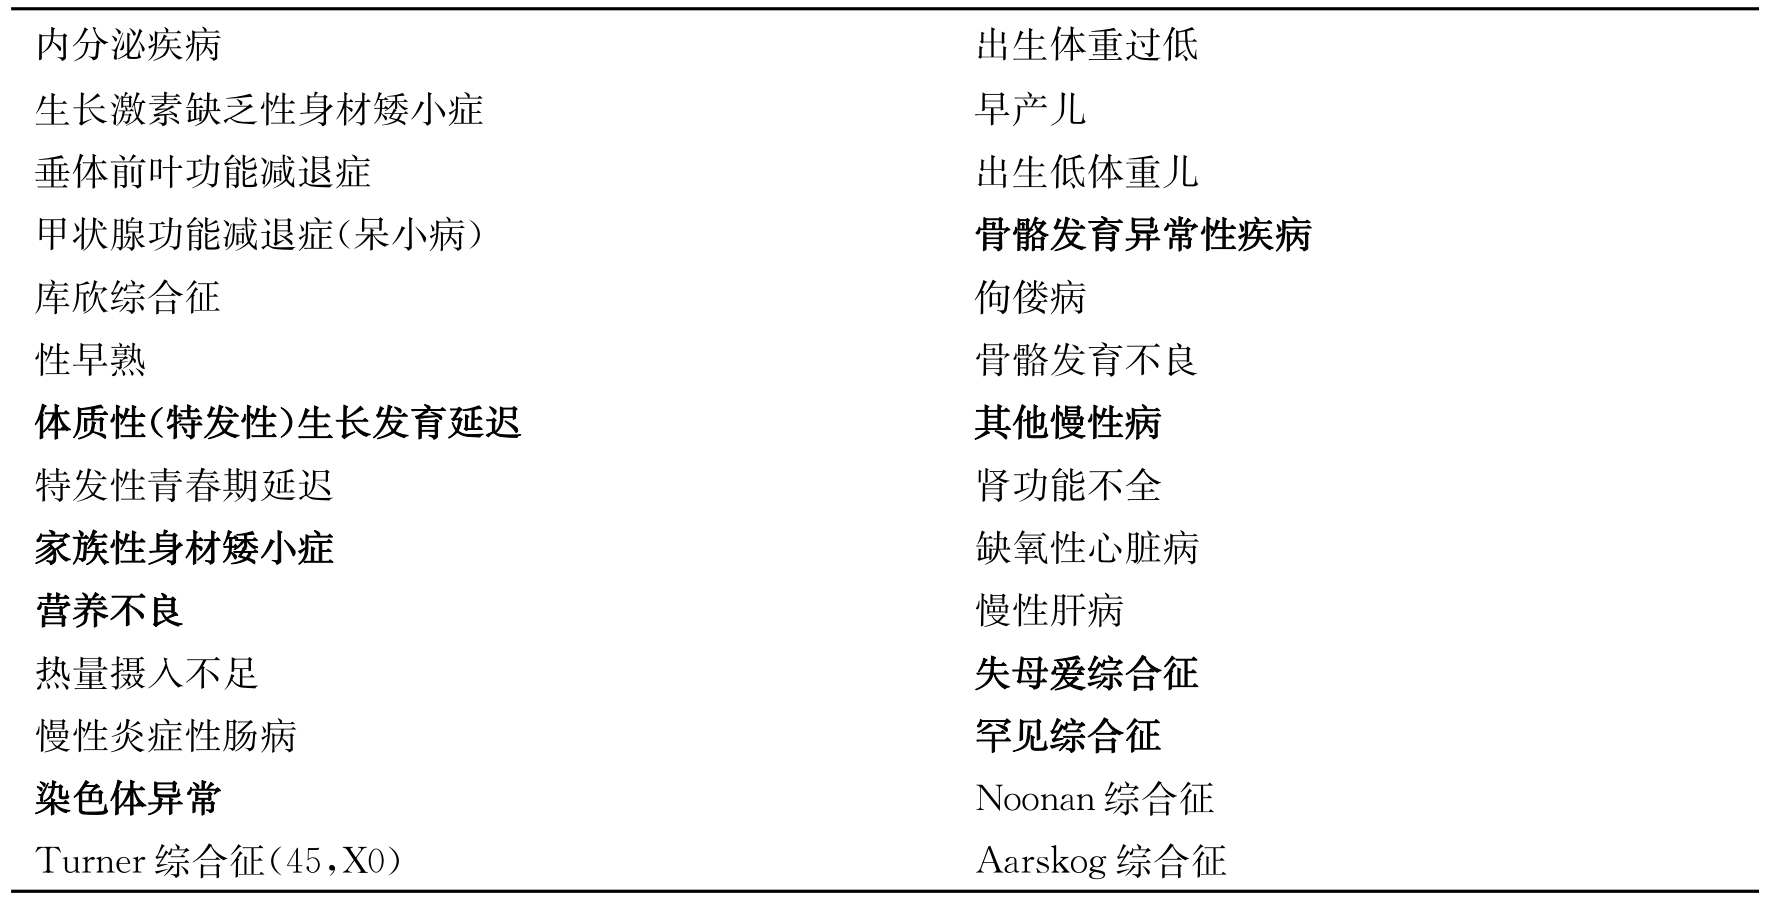
\includegraphics[width=5.91667in,height=3.03125in]{./images/Image00249.jpg}
\end{table}

\subsection{一、内分泌疾病}

\subsubsection{(一)生长激素缺乏性身材矮小症}

单纯生长激素缺乏引起的矮小体型,旧称垂体性侏儒症,通常患儿在出生时身长、体重与正常新生儿无异,但在出生后第一个生长高峰内身高增长的速度即开始落后,细心的家长往往在患儿2~3岁甚至更早时发现孩子身高矮于同龄儿,若此时未予诊断及干预,随着年龄的增长,身材矮小表现更为突出。患儿智力发育一般不受影响,进入青春期后,由于生长激素与性激素存在协同作用,生长激素缺乏也会影响性激素的作用,患者青春期启动年龄往往较正常延迟,但最终部分患者第二性征发育完全,可正常生育,性成熟后骨骺闭合,故成年后身高一般不超过1.3m。

体征方面除体型矮小外,患者身材匀称协调,至成人后仍可保持儿童外貌,面颊圆形丰满(因生长激素缺乏,脂肪动员减少所致),皮肤细腻干燥有皱纹,皮下脂肪丰满,第二性征发育虽差且落后于正常,但多数患者最终可发育完全。实验室检查方面,对疑诊生长发育迟缓患者需常规进行骨龄测定(非优势手腕摄片),可见骨龄落后于实际年龄。由于生长激素呈脉冲式分泌,峰值与谷值相差较大,正常人生长激素分泌谷值与实际缺乏者无法区分,故不能仅凭基础生长激素值诊断本病,需进行生长激素兴奋试验。常用的兴奋试验包括胰岛素低血糖试验、精氨酸兴奋试验、左旋多巴试验、可乐定试验、生长激素释放激素兴奋试验等。如刺激后生长激素峰值>10μg/L为正常,<5μg/L为反应低下,若为两者之间则提示部分缺乏。一般需要两种不同的生长激素兴奋试验结果一致才诊断为生长激素缺乏症。另外,IGF-1及IGF结合蛋白-3(IGFBP-3)可较恒定地反映生长激素分泌水平,两者一般随年龄而升高,于青春发育中期(女孩11~12岁,男孩13~14岁)达高峰,随后逐渐下降至成人水平。垂体影像学检查(包括MRI或CT)有助于排除颅内占位病变,需注意垂体的高度和体积、垂体柄的位置以及垂体后叶高信号等情况,判断是否存在先天性垂体发育不良等。

上海市儿科研究所提出的生长激素缺乏性身材矮小症的诊断标准如下:①身高低于同年龄、同性别正常人2个标准差或第3百分位;②生长速率<4cm/年;③骨龄落后于同年龄、同性别正常人均值2年以上;④三种生长激素激发试验血生长激素峰值<10μg/L;⑤排除引起生长迟滞的其他疾病。

\subsubsection{(二)垂体前叶功能减退症}

狭义的垂体前叶功能减退症是指由于肿瘤、炎症、先天发育缺陷等因素导致垂体多种促激素分泌缺乏所引起的继发性靶腺功能减退症;广义则包括单一腺垂体激素分泌不足的情况。垂体后叶多不受累,一般无尿崩症表现。由于垂体前叶功能减退症所致身材矮小症主要因生长激素与性激素同时缺乏引起,一般生长激素缺乏表现较早,智力受损不突出,由于性激素分泌不足,青春期启动明显延迟,第二性征发育较单纯生长激素缺乏症者更差,无青春期身材激增表现。由于性激素缺乏骨骼闭合延迟,成年后身高仍缓慢增长,故就诊时身高常超过1.3m,甚至随着年龄的增长,最终身高并无明显落后。若合并促甲状腺激素分泌不足,甲状腺功能减退症的表现相对较轻,一般不出现黏液性水肿及呆小病表现。合并促肾上腺皮质激素分泌不足,常表现为皮肤白皙、体型消瘦、精神及体力较差,长期进食较少、偏食,故而营养状态较差,非应激状态下一般不出现肾上腺危象。

体检儿童外貌,身材矮小消瘦,皮肤较白,下部量长于上部量,两指间距长于身高,第二性征发育差,外生殖器幼稚。

实验室检查提示骨龄落后,长骨骨骺未闭,除生长激素兴奋试验显示生长激素不被激发以及IGF-1和IGFBP-3水平较低外,促性腺激素释放激素(GnRH)兴奋试验显示黄体生长素(LH)及促卵泡激素(FSH)基础分泌显著降低,且不被GnRH兴奋(包括兴奋的倍数及兴奋后的绝对值极低)。

垂体影像学检查有助于病因诊断。

\subsubsection{(三)甲状腺功能减退症(呆小病)}

甲状腺激素缺乏引起的矮小体型多为原发性甲状腺功能减退症所致,常于出生后数周或婴幼儿期起病,起病越早,病情越严重。因伴有神经系统不可逆性损伤,智力受损明显,患儿有特殊外貌,旧称“呆小病”或“克汀病”。既往主要见于地方性甲状腺肿流行区,因母体缺碘而导致胎儿碘缺乏,甲状腺发育不全和甲状腺素合成不足。食盐加碘后呆小病多为散发,见于多种原因所致甲状腺发育不全或缺如,以及甲状腺素合成障碍性疾病,包括:①甲状腺先天性缺如或发育缺陷;②母体存在抗甲状腺抗体,通过胎盘破坏胎儿甲状腺;③妊娠期服用抗甲状腺药物阻碍胎儿甲状腺的发育和甲状腺素的合成;④异位甲状腺;⑤促甲状腺激素受体基因突变所致促甲状腺激素不敏感;⑥碘泵(NIS)基因突变导致甲状腺浓集碘功能障碍。

患儿体型矮小、智力发育迟钝、表情呆滞、声音低哑、颜面苍白水肿、眼距增宽、鼻梁扁塌、唇厚流涎、舌大外伸、囟门增大、关闭延迟,出牙、换牙延迟,骨龄落后于实际年龄,行走晚、呈鸭步、心率慢、性发育延迟。

实验室检查可有贫血,为正常细胞型正常色素性贫血,甲状腺功能提示T3、T4降低,TSH明显升高。甲状腺B超有助于了解甲状腺大小、形态,有无缺如,甲状腺核素扫描可发现异位甲状腺(舌骨后、胸骨后、纵隔内、卵巢等)。

\subsubsection{(四)库欣综合征}

库欣综合征是各种病因引起肾上腺分泌过多糖皮质激素(皮质醇)所致病症的总称,分为依赖促肾上腺皮质激素(ACTH)的库欣综合征(库欣病及异位ACTH综合征)以及不依赖ACTH的库欣综合征(肾上腺皮质腺瘤、肾上腺皮质腺癌、不依赖ACTH的双侧肾上腺小结节性增生、不依赖ACTH的双侧肾上腺大结节性增生)。

儿童期起病的库欣综合征,由于过量皮质醇可抑制生长激素的分泌及作用,并能直接影响性腺以及抑制促性腺激素的分泌,故对生长发育有严重影响。另外,糖皮质激素具有降低骨胶原转换的作用,影响小肠对钙的吸收,促进骨钙动员,大量钙离子进入血液后从尿中排出,从而导致继发性骨质疏松,严重者可诱发脊椎压缩性骨折,使身材更矮。患儿除矮小体型外,往往伴有向心性肥胖、满月脸、水牛背、锁骨上窝脂肪垫、皮肤薄、可见散在瘀斑、紫纹等典型库欣外貌。另外,患儿还可伴高血压、电解质紊乱(高钠、低钾碱血症、低钙血症)、糖耐量异常等表现。

实验室检查提示血、尿皮质醇浓度明显升高,失去昼夜节律,且不被外源性地塞米松所抑制,即可拟诊库欣综合征。ACTH浓度测定有助于区分是否依赖ACTH,垂体及肾上腺影像学检查利于病因及定位诊断,大剂量地塞米松抑制试验可鉴别库欣病还是其他病因所致库欣综合征,岩下窦采血测ACTH与外周血ACTH比较,是鉴别不典型、缓慢进展的异位ACTH综合征与库欣病的金标准。

\subsubsection{(五)性早熟}

男孩在9岁前、女孩在8岁前出现性腺增大和第二性征发育称为性早熟,可分为中枢性性早熟和周围性性早熟两大类。中枢性性早熟又称为GnRH依赖性或真性性早熟,系下丘脑-垂体-性腺轴不适当地过早解除抑制,青春期提前启动,患儿表现与正常性发育期相同,第二性征与遗传性别一致,能产生精子或卵子,具有生育能力。病因包括特发性性早熟以及中枢神经系统疾病(包括中枢系统肿瘤及非肿瘤性因素)所致性早熟。周围性性早熟又称非GnRH依赖性或假性性早熟,是由性腺中枢以外的因素产生过多的性激素,或因外源性因素导致血中性激素水平升高所致,通常只有第二性征的发育,而生殖细胞并未同步成熟,不具备生育能力。病因包括分泌促性腺激素的肿瘤(如绒癌、畸胎瘤、肝脏肿瘤等)、睾丸Leydig细胞瘤或肾上腺病变导致雄激素产生过早过多、McCune-Albright综合征、饮食等外源性因素导致性激素摄入过多等。患儿性发育始于正常性发育前的任何年龄,第二性征发育次序与正常儿童一致,但发育提前、速度加快,性心理成熟也更早,同时伴有身材激增,骨龄提前,但由于性激素促进骨骺过早闭合,使患者到成年时身材反而矮于正常人。

\subsection{二、体质性(特发性)生长发育延迟}

体质性(特发性)生长发育延迟约占儿童矮小体型患者的30\%,尤其是来自偏远山区、经济落后的农村地区的身材矮小症儿童绝大多数属于此类,且男孩更为多见。患儿出生时身长、体重均正常,此后生长缓慢,逐渐落后于同龄正常儿童,骨龄亦延迟2年以上,但无明确垂体疾病及其他慢性疾病的证据。患儿通常智力正常,青春期启动延迟,可延至16~17岁才开始第二性征发育。一旦青春期启动,生长速度加快,肌肉逐渐发达,性发育和骨骼发育也将快速追赶同龄人,由于骨骺闭合较迟,最后身高和性成熟都可达到成人正常水平。

体质性(特发性)青春期延迟机制未明,因许多患者的直系亲属也有青春期发育延迟表现,故推测可能与基因遗传有关;大部分患者体型偏瘦,也有认为可能与机体能量储备不足有关;近期还有研究提示,体质性(特发性)青春期延迟患者的基础代谢率高于普通人群,推测能量负平衡可能是导致青春期延迟的原因;另外,全身性疾病和营养不良患者,在原发疾病和营养状态改善后可出现正常性发育,推测青春期发育延迟可能和疾病相关的炎症介质作用于中枢神经系统,从而抑制下丘脑-垂体-性腺轴的启动有关。

\subsection{三、家族性身材矮小症}

正如前述,人体身高75\%取决于遗传因素,父母身材矮小,子女预期的身高也会偏矮,由于遗传因素引起的矮小体型称为“家族性身材矮小症”,通常患儿出生时身长较短,此后生长速度可正常,生长曲线与正常儿童的生长曲线平行,但始终低于参考人群的第3百分位数,成年后最终身高与生父母相似。无明确的器质性病变,骨龄与实际年龄相符,生长激素及IGF-1、IGFBP-3水平正常,青春期启动无延迟,第二性征发育及生育能力不受影响,无需特殊治疗。

\subsection{四、营养不良}

儿在生长发育期内由于地区或家庭经济落后、环境因素等原因,无法获得充足的食物,或由于自身慢性疾病或慢性感染(包括结核、寄生虫等)影响食欲,导致热量摄入不足,或由于慢性炎症性肠病引起胃肠消化吸收功能障碍、慢性腹泻等,均可导致生长发育所需能量、蛋白质、电解质、维生素、微量元素等严重缺乏而影响生长发育。患儿身材矮小瘦弱,体型匀称,智力一般无明显影响,出牙换牙迟,牙齿骨骼发育不良,青春期启动延迟,第二性征发育差。严重营养不良者还可伴全身水肿、腹水。补充足够热量或治愈慢性疾病后,生长发育情况常得以改善。

\subsection{五、染色体异常}

引起矮小体型的病因中,Turner综合征并不少见,为X染色体单体(45,X0)或X染色体结构异常所致疾病,部分患者染色体核型为嵌合体,如45,X0/46,XX、45,X0/47,XXX、45,X0/46,XY、45,X0/46,XX/47,XXY等。

患者体型矮小,成年身高一般不超过1.5m,往往出生前有宫内生长迟缓史,出生时身长较短,3岁以后生长明显缓慢,身高增长落后于正常生长曲线,于青春期年龄无身材激增,智力发育多不受影响。可伴有特殊面容,如眼距宽、鼻梁扁塌、下颌小、牙床发育不良、通贯掌、皮肤多黑痣。半数患者可有颈蹼、颈较粗短、发际低,部分患者有肘外翻,可合并心血管畸形。性腺发育不全是其突出表现,原发性闭经,第二性征发育不全,乳房及乳头未发育,乳距宽,无阴毛及腋毛,子宫缺如或始基子宫、卵巢呈条索状或发育不良。本病为原发性性腺功能减退症,故雌激素显著降低,而LH和FSH明显升高,染色体核型分析可确诊本病。

\subsection{六、出生体重过低}

出生体重<2500g称为低体重儿,<1500g为极低体重儿。胎龄在37周以前出生的活产婴儿为早产儿,出生体重大多在2500g以下。早产的原因往往存在胎盘因素或母体疾病等,使胎儿未能在宫内充分发育完全就出生,器官功能不完善,适应能力较差,出生后吸奶无力,进食量不足,对感染抵抗力低,能量消耗大,从而使出生后的生长追赶不足,故在生长发育期可落后于同龄人。胎儿在宫内的生长发育主要取决于IGF-1及IGF-2的作用,两者通过IGF-1受体促进宫内生长,在孕晚期IGF-2还可部分依赖胰岛素受体发挥调节生长发育的作用。已有文献报道,存在IGF-1受体或胰岛素受体基因突变的患儿,即使足月出生也可表现为出生体重过低,出生后生长追赶不足,从而导致矮小体型及青春期启动延迟。孕母妊娠生产史及出生后生长追赶情况的问询有助于病因判断。

\subsection{七、骨骼发育异常性疾病}

体型的高矮主要取决于骨骼发育的情况,任何导致骨骼发育异常的疾病,若起病时间在幼年、骨骺尚未闭合前均可影响身材的增长。维生素D缺乏可引起钙、磷代谢异常,骨组织钙化不良,骨骼生长障碍。儿童期、骨骺闭合前起病的维生素D缺乏称为佝偻病,患儿往往体型矮小、伴神经精神症状(如烦躁、易激惹、睡眠不宁)、低钙抽搐、骨骼发育异常(如颅骨软化、囟门关闭延迟、胸部肋串珠、鸡胸、漏斗胸、O型腿或X型腿)等表现。实验室检查显示25-OH维生素D降低、碱性磷酸酶增高、血钙、血磷浓度降低,X线片显示不同程度的佝偻病改变。其他婴幼儿起病、引起骨骼发育不良的疾病还包括肾小管酸中毒、甲状旁腺功能减退症(包括先天性及假性甲旁减等)、低血磷性抗D佝偻病、多发性骨纤维结构不良、成骨不全等。

\subsection{八、其他慢性病}

维生素D需分别在肝脏的25-羟化酶及肾脏的1-羟化酶作用下活化,才能发挥调节钙磷代谢的作用,故婴幼儿期起病的慢性肝病,以及慢性肾脏疾病所致肾功能不全均可抑制维生素D的活化而影响钙磷代谢,此外疾病本身伴发的胃纳减少、腹泻等症状也可影响维生素D及钙、磷、蛋白质的摄取与吸收,或致骨转换所需原料丢失过多,均可影响骨骼的发育及身材的增长。严重的先天性缺氧性心脏病,幼年起病,脑组织供血不足,垂体缺血缺氧将影响生长激素、性激素的分泌,从而导致生长发育迟缓,体型矮小,青春期启动延迟。此类躯体慢性疾病所致身材矮小症,由于原发病突出的临床表现,病因诊断不难,身材矮小反而容易被忽略。

\subsection{九、失母爱综合征}

属于心理社会性矮小症的一种,是指婴幼儿期母爱被完全剥夺后,患儿的精神、心理、情感受到严重创伤,这种心理社会应激反应将影响大脑皮质向下丘脑的神经冲动传递,从而抑制生长激素释放激素的分泌,故患儿的生长激素、IGF-1、IGFBP-3分泌减少,生长激素不被兴奋。患儿遗传的体格生长和精神发育的能力正常,改变环境因素,有效的心理辅导后可获得恢复。

\subsection{十、罕见综合征}

\subsubsection{(一)Noonan综合征}

又称先天性侏儒痴呆综合征,是一种常染色体显性遗传病,通常染色体核型正常,患儿除矮小体型、智力低下外,往往有特殊面容,包括眼睑下垂、眼距增宽、鼻梁扁塌、小下颌、牙齿异常、颈蹼、后发际低,鸡胸或漏斗胸、肘外翻、生殖器发育不良等,大多数患儿合并心血管畸形,以肺动脉狭窄和房间隔缺损较多见。临床表现与Turner综合征相似但核型正常,也称作假性Turner综合征。

\subsubsection{(二)Aarskog综合征}

是罕见的X染色体连锁隐性遗传病,患儿出生时身长可正常,在青春期前保持矮小体型,但血清生长激素水平正常,青春期启动常延迟,但启动后可有身材激增,成年后身高可达参考人群第10百分位数。患儿常伴有特殊面容,包括圆脸、上颌发育不良、宽鼻梁、短指、并指畸形、关节过伸、拇指外展受限、淋巴水肿、阴囊包绕阴茎、大睾丸、尿道下裂、腹股沟疝、隐性脊柱裂、脊柱侧弯畸形等。

\protect\hypertarget{text00314.html}{}{}

\section{134 肥胖}

肥胖系指体内贮积的脂肪含量超过理想体重20\%以上。用于体脂测量的指标很多,常用的包括体重指数(BMI=体重(kg)/身高2(m))、腰围(测量周径经过肋骨下缘最低点与髂嵴最高点连线的中点)、腰臀比、腰身比、皮褶厚度、臂周长、双能X线吸收法(DEXA)、身体密度测量法等。用于皮下和腹部脂肪测定的方法包括超声波、红外线、CT、MRI等。

根据2011年《中国成人肥胖症防治专家共识》,BMI仍是目前临床上最常用的衡量肥胖程度的简易指标,中国人BMI在24.0~27.9kg/m\textsuperscript{2}
之间为超重,≥28.0kg/m\textsuperscript{2}
为肥胖。专家共识同时指出,在不同个体,某一BMI水平并不总是意味着相同的肥胖程度,尤其是对肌肉特别发达的个体,BMI并不能准确地反映肥胖的程度。腰围是反映腹型(或中心性)肥胖的重要指标,WHO建议亚太地区男性>90cm,女性>80cm作为腹型肥胖的标准,国内研究显示,对于中国人男性腰围>90cm,女性腰围>85cm可能是一个更为合适的切点。

肥胖症根据病因可分为单纯性肥胖与继发性肥胖。前者是指肥胖的病因不明,除肥胖所致并发症外,一般不伴器质性疾病,在病因构成中占大部分,但诊断时需首先排除继发性肥胖的病因,属于排他性诊断。

病史询问时需关注出生时体重、肥胖起始的年龄、体重增长的速度、父母及近亲有无肥胖史、饮食运动睡眠习惯、职业及经济状况、有无吸烟及戒烟、月经、生育及绝经情况。需鉴别的继发性肥胖所特有的症状、肥胖症相关并发症及合并症(如睡眠呼吸暂停、肺通气减低综合征、退行性关节炎、高血压、糖尿病、痛风等)情况。

体格检查方面包括身高、体重、BMI(可据此判断肥胖的程度)、腰围、腰臀比、腰身比,全身性还是向心性肥胖、腹型肥胖还是均匀性肥胖;第二性征特别是外生殖器发育情况,有无满月脸、多血质外貌、水牛背、锁骨上窝脂肪垫、皮肤紫纹及瘀斑;有无颈项部皮肤黑棘皮征、多毛、痤疮、男性化表现;有无水肿、贫血外貌、上睑下垂、腱反射减弱而恢复期延长;有无黄色瘤、巨舌、肌无力,有无先天性心脏病特有的心脏体征等。

继发性肥胖需考虑以下疾病:

\subsection{一、库欣综合征}

由于血中皮质醇浓度升高可促进食欲,从而导致患者体重增加。皮质醇拮抗胰岛素作用而继发高胰岛素血症,后者可引起水钠潴留及脂肪合成增多,但脂肪聚积呈向心性分布。多数患者为轻至中度肥胖,极少数为重度肥胖,有时患者体重并无增加,而表现为面部及躯干脂肪积聚而四肢变细。大多数患者因具有典型的库欣外貌(向心性肥胖、多血质、皮肤瘀斑、紫纹、皮肤变薄、水牛背、锁骨上窝脂肪垫等)而获得拟诊,结合患者伴高血压、糖耐量减低、电解质紊乱(低钾碱血症)、继发性骨质疏松症、皮肤真菌病等,通常不难诊断。进一步确诊及病因、定位诊断需依赖实验室检查,譬如24小时尿游离皮质醇或17-OH皮质类固醇升高,血皮质醇浓度升高且失去昼夜节律,不被外源性小剂量地塞米松所抑制,即可诊断为皮质醇增多症;检测血ACTH可鉴别是否为ACTH依赖性的库欣综合征,依赖性者ACTH水平升高,非依赖性者ACTH常明显抑制。ACTH依赖性库欣综合征包括库欣病及异位ACTH综合征;非ACTH依赖性库欣综合征则包括肾上腺皮质腺瘤或癌、非ACTH依赖性的双侧肾上腺大/小结节性增生等。

库欣病与典型的异位ACTH综合征的ACTH水平往往有明显差异,后者通常血浆ACTH浓度显著升高>66pmol/L,而库欣病一般为轻至中度升高。大剂量地塞米松抑制试验(8mg/d)有助于库欣病与其他病因引起的库欣综合征相鉴别,国外研究约85\%库欣病能被抑制到低于基础水平的50\%,而根据中山大学附属第一医院的资料显示约28\%库欣病不能被大剂量地塞米松所抑制。临床上最难鉴别的是库欣病与支气管类癌等引起的缓慢进展型异位ACTH综合征,此时可考虑行岩下窦采血,测定垂体静脉与外周静脉血ACTH浓度比值,采血前注射促肾上腺皮质激素释放激素(CRH)可提高诊断准确率,一般比值>3提示为库欣病,<1.8则考虑异位ACTH综合征。

此外,根据病因构成、患者的发病年龄、性别等,有时也可为库欣综合征的病因判断提供部分线索:

1.库欣综合征的病因构成东西方差异较大,但库欣病仍是最常见病因,国外文献显示其发病率是肾上腺皮质腺瘤及癌引起库欣综合征总和的5~6倍,而异位ACTH综合征是第二常见的病因。中山大学附属第一医院统计近10年共154例临床确诊的库欣综合征,其中库欣病占53.2\%,肾上腺皮质腺瘤占33.8\%,肾上腺皮质腺癌占1.94\%,异位ACTH综合征占5.84\%。异位ACTH综合征患者的库欣体征常不典型,易被原发肿瘤伴随的临床表现所掩盖,且因原发病就诊手术科室而漏诊伴发的内分泌疾病,可能是造成国内外资料差异的主要原因。

2.女性发生库欣病是男性的3~8倍,合并肾上腺良、恶性肿瘤是男性的3倍,其中伴库欣综合征的肾上腺皮质腺瘤是男性的4~5倍;既往男性发生异位ACTH综合征是女性的3倍,但近年由于女性吸烟导致肺癌比例上升,异位ACTH综合征的性别比例差距也在缩小。

3.异位ACTH综合征和肺癌发病率随年龄增长而上升,在50岁以后迅速达高峰;库欣病在20~45岁之间发病率最高;肾上腺皮质腺瘤和癌发病呈双峰,第一个小高峰是在20岁以前,另一个明显的发病率高峰在腺瘤为50岁以后,而在腺癌则为40岁以后。

\subsection{二、多囊卵巢综合征}

又称为Stein-Leventhal综合征,是育龄期女性较常见的引起肥胖、月经紊乱、不孕不育的原因。据文献资料,多囊卵巢综合征患者合并肥胖者约占30\%~60\%,甚至可高达75\%。多囊卵巢综合征的病因及发病机制未完全清楚,一般认为与下丘脑-垂体-性腺轴功能紊乱有关,主要病理生理基础是胰岛素抵抗,后者是引起患者肥胖的主要原因。

患者的临床表现包括:体型肥胖、月经紊乱(如月经稀发、闭经)、多毛、面部皮脂分泌较多、痤疮、声音低粗、阴蒂肥大和喉结等男性化表现、长期不排卵可致不孕。由于胰岛素抵抗,多囊卵巢常作为代谢综合征的组分,可合并高血压、糖耐量减低、痛风、血脂异常、阻塞性睡眠呼吸暂停等,合并肿瘤的风险也明显增加。

实验室检查表现为血浆睾酮、脱氢异雄酮升高,雌二醇降低、LH/FSH比例升高(常≥2.5~3),经直肠或阴道盆腔B超检查显示“卵巢多囊样改变”(双侧卵巢增大,被膜增厚回声强,被膜下可见直径2~9mm囊状卵泡,每个平面至少有12个以上卵泡,围绕卵巢周边呈车轮状排列,称为项链征,卵巢间质回声不均,子宫内膜增厚等)。

目前临床上常用于诊断多囊卵巢综合征的仍然是2003年5月欧洲人类生殖和胚胎学会与美国生殖医学会(ESHRE/ASRM)提出的诊断标准:

(1)超声存在多囊卵巢;

(2)临床或实验室检查提示高雄激素血症;

(3)无排卵性月经紊乱。

符合上述3项中的2项,且排除其他病因者可诊断为多囊卵巢综合征。

\subsection{三、胰岛素瘤}

胰岛素瘤源于胰岛β细胞,是内源性高胰岛素血症引起低血糖症中最常见的原因之一。患者胰岛素的分泌水平未必比正常人显著升高,但常合并肥胖,此系胰岛素反复不适当分泌增多,导致血糖显著降低,机体能量不足,迫使患者增加防御性进食所致。胰岛素瘤患病率低,约8~9/10万,各年龄段均可发病,高发年龄为30~60岁,女性稍多,少数可为家族性多发性内分泌腺瘤综合征I型(MEN-I)的组分。成人胰岛素瘤单个常见,90\%以上为良性。大多数儿童及个别成人可无肿瘤,而以细胞增生为主(胰岛β细胞增生症)。

胰岛素瘤突出的临床表现为低血糖症,多发生于清晨或黎明前空腹状态,低血糖症状常由轻渐重,由偶发至频发,逐渐加重及频密,发作频率取决于肿瘤分泌胰岛素量及机体对低血糖的耐受性、有无防御性进食加餐等;发作时症状的出现也与血糖下降的速度及持续的时间、发作的频次有关。初起病时患者常有饥饿、头晕、乏力、冷汗、心悸等交感神经兴奋表现,随着低血糖持续频繁发作,患者对低血糖感知力削弱而耐受性增加,交感神经兴奋表现可不明显,而以中枢神经系统缺糖而引起的神经精神症状为主,表现为思想难集中、思维及语言迟钝、感觉与行为异常、妄想、痴呆,可被误诊为精神分裂症;个别严重病例可出现癫痫样抽搐,常被误诊为癫痫。久病者常有智力、记忆力和定向力障碍。

诊断胰岛素瘤需有低血糖时内源性胰岛素不适当分泌增多的证据,临床上常用胰岛素释放指数,即低血糖症时血浆免疫反应性胰岛素(IRI,mU/L)与同步血浆葡萄糖(mg/dl)的比值。正常人<0.3,胰岛素瘤患者95\%比值>0.3,若比值>0.4则基本可以肯定诊断。疾病早期低血糖呈间歇性发作的,可通过72小时饥饿试验诱发低血糖症的出现。其他检查包括修正的胰岛素释放指数、血清C肽测定、血清胰岛素原测定、胰高糖素激发试验、亮氨酸试验等也有助于明确内源性胰岛素分泌与低血糖症的关系。定位诊断常采用薄层胰腺CT或腹部B超、腹腔选择性动脉造影、超声胃镜、PET-CT等,对于难以定位的病例有时需腹腔探查,结合术中超声或术中胰静脉插管分段采血检测胰岛素浓度而获得诊断。

\subsection{四、下丘脑性肥胖}

常见于下丘脑综合征患者,此系各种致病因素累及下丘脑,使其结构、代谢及功能受损而引起的临床综合征。病因包括先天性损伤及遗传性因素、肿瘤、炎症与感染、肉芽肿、退行性变、血管损伤、手术、代谢性疾病、药物及下丘脑功能性障碍等。临床表现为下丘脑功能紊乱及神经精神症状。下丘脑功能紊乱可累及睡眠中枢、食欲中枢和体温中枢,患者可表现为嗜睡或失眠、多食肥胖或厌食消瘦、体温过高或过低、精神障碍、头痛、多汗。故以嗜睡、多食为主要表现的下丘脑综合征患者,多为肥胖体型。

临床上遇到下列线索时需考虑下丘脑综合征可能:①内分泌症状及体征不能用单一的靶腺或单纯垂体损伤解释;②内分泌功能紊乱症状伴肥胖、嗜睡、多食或消瘦、失眠、厌食,精神失常或体温异常,无其他原因解释;③颅内压增高伴视力下降、视野缺损,或伴尿崩症、性腺功能减退、溢乳等;④伴发育不良、嗅觉障碍、畸形或性腺发育不良者;⑤体质虚弱,尤其伴血皮质醇降低或自身免疫病者;⑥低T\textsubscript{3}
/T\textsubscript{4} 综合征。

下丘脑性肥胖多为均匀性肥胖,可伴下丘脑功能紊乱的其他临床表现,如睡眠(嗜睡)、进食(多食)障碍、体温调节障碍、自主神经功能紊乱、尿崩症、女性月经失调或闭经,男性性功能减退等。此外,若因肿瘤或感染引起者,可伴相应肿瘤压迫症状及全身性感染表现。实验室检查方面需进行垂体前叶各条轴(肾上腺皮质、甲状腺、性腺)的功能评估,垂体后叶功能学检查(尿比重、尿渗透压、禁水加压素试验)、自主神经功能检查、GnRH兴奋试验、CRH兴奋试验、TRH兴奋试验,垂体MRI检查有利于了解下丘脑及垂体占位病变情况。

\subsection{五、甲状腺功能减退症}

甲状腺功能减退症(甲减)患者常因代谢率降低、思睡懒动,机体消耗减少而导致体重增加,严重者伴发黏液性水肿,则体重进一步上升导致肥胖的发生。甲减合并肥胖体型者多见于原发性甲减,继发性甲减常伴低促性腺激素性性功能减退、继发性肾上腺皮质功能减退,一般体重减轻,出现黏液性水肿也罕见。原发性甲减的病因最常见桥本甲状腺炎、甲亢\textsuperscript{131}
I治疗后、甲状腺手术、颈部放射治疗、甲状腺晚期癌或转移瘤、抗甲状腺药物过量等。临床表现为乏力、怕冷、胃纳减、便秘、体重增加、思睡、贫血、皮肤干燥粗糙,女性常有月经量增多、经期延长,合并黏液性水肿者皮肤呈非凹陷性水肿。甲状腺功能检查提示T\textsubscript{3}
、T\textsubscript{4}
降低,TSH明显升高即可诊断为原发性甲减。抗甲状腺抗体(TRAb,TPOAb,TGAb)显著升高有助于桥本甲状腺炎的诊断。

\subsection{六、肥胖-生殖无能综合征}

体型显著肥胖者常影响性能力、月经或生精功能而导致生育困难,体重减轻后生育能力常获改善。肥胖-生殖无能综合征特指某些病变(肿瘤、炎症、血管病变、脑外伤等)累及下丘脑,导致神经-内分泌功能紊乱,引起GnRH分泌减少、继发性性腺发育不良及脑性肥胖,又称为Fröhlich综合征、脑性肥胖症或Barbinski-Fröhlich综合征。

多于儿童或青少年起病,男性多于女性。肥胖是由于食欲亢进,食量增加所致,多呈均匀性,有时为向心性,由于脂肪过多堆积,男性乳房外形似女性型(非乳腺增生症),女性患者则乳房更丰满。性腺功能减退表现为性腺发育不良,男性阴茎短小、睾丸小而软或为隐睾;女性外阴不发育,子宫发育不良,无月经,男女患者第二性征均缺如。少数成年起病者可有生殖器萎缩、性毛脱落、阳痿或闭经表现。此外,本病还可伴下丘脑功能紊乱表现(睡眠障碍、体温调节异常、中枢性尿崩症及自主神经功能失常等)以及原发病因相关的临床表现。

\subsection{七、性腺功能减退所致肥胖}

女性绝经后易发生肥胖,此与雌激素浓度降低、胰岛素抵抗,以及围绝经期自主神经功能紊乱、饮食运动习惯改变等有关。男性睾丸功能减退或完全丧失后也容易发生肥胖。此类肥胖多为中度,重度肥胖者少见。除肥胖外,患者主要表现为第二性征萎缩退化、阴茎变小、声音尖细,女性阴道萎缩,皱褶减少或消失,阴道分泌物减少。实验室检查提示男性睾酮降低,女性雌、孕激素均降低,FSH、LH明显升高,对GnRH反应过度。

\subsection{八、药 物}

很多药物可以引起肥胖,如糖尿病患者长期使用磺脲类口服降糖药、胰岛素,肾病综合征或系统性红斑狼疮患者长期使用超生理量糖皮质激素,抗精神病药物如氯氮平、奥氮平、氯丙嗪、奋乃静等。结合患者原发疾病史及用药史,一般诊断不难。

\subsection{九、泌乳素瘤}

泌乳素瘤患者可出现肥胖(男性肥胖发生率约69\%),主要由于慢性高泌乳素血症引起下丘脑-垂体-性腺轴功能受抑制,下丘脑GnRH及垂体LH,FSH分泌减少所致继发性性腺功能减退。肥胖多为轻度、均匀性,此外高泌乳素血症可引起女性月经减少、闭经、溢乳、不孕不育,男性阳痿、性功能减退等表现。肿瘤大者还可伴压迫症状,如头痛、视力下降、视野缺损。血浆泌乳素水平显著升高,垂体CT或MRI发现占位病变即可诊断。

\subsection{十、痛性肥胖}

女性患者多见,在绝经后发病,肥胖主要集中在躯干、颈部、腋部,脂肪沉积处可有触痛,且可触及小结节,肌力低下,患者易感疲劳,可伴抑郁、痴呆、癫痫等。实验室检查无特殊,诊断主要依赖临床表现。

\subsection{十一、糖原贮积症}

糖原贮积症是由于糖原合成和分解所需的酶存在遗传性缺陷而引起的罕见综合征,大多数为常染色体隐性遗传,个别为X染色体伴性遗传。因为涉及糖原合成途径的多个酶,不同的酶缺陷可致不同临床亚型,临床表现各异,但低血糖症和(或)肌无力是所有亚型共有的临床特点。本病多发生于婴、幼儿和青少年,肥胖多因进食多所致,可伴肝大、心脏增大、黄色瘤、巨舌等表现。实验室检查提示低血糖症、高甘油三酯、高尿酸、高乳酸血症,肾上腺素或胰高糖素刺激无血糖升高反应,肝脏或肌肉活检有助于诊断。

\subsection{十二、颅骨内板增生症}

属于遗传性疾病,仅见女性发病,多于绝经后期发病,肥胖通常以躯干和四肢近端为主,可伴剧烈头痛。颅骨X线摄片见颅骨内板增生即可确诊。

\subsection{十三、其他罕见的综合征}

\subsubsection{(一)Carpenter综合征}

患儿表现为肥胖、智力迟滞、尖脑、眼距增宽、斜视、眼球突出、视乳头水肿、视力下降、内眦赘皮、多指及并指畸形、髋外翻、膝、足内翻、脐疝、性功能减退、先天性心脏病(如动脉导管未闭)等表现。颅骨X线摄片可见颅骨变薄,有显著的“指压痕”,骨缝纹痕消失,骨盆呈漏斗状,尿液分析可有氨基酸尿。

\subsubsection{(二)Cohen综合征}

为常染色体隐性遗传病,患儿体型轻度肥胖,小眼睛、小脑袋,呈先天性愚型眼型,严重者智力迟钝,可有斜视、近视、小颌、腭弓狭窄高耸、呈猿样皮纹,并指、关节过伸、膝内翻、脊柱侧弯、肌张力减低。脑电图表现为弥漫高波峰。

\subsubsection{(三)Prader-Willi综合征}

属于遗传性疾病,患儿表现为肥胖、身材矮小、性腺功能减退、体格发育及第二性征发育延迟,荧光原位杂交检出染色体15q11-13存在间质性微缺失即可确诊。

\subsubsection{(四)Aström综合征}

为常染色体隐性遗传病,儿童期起病,表现为肥胖、色素性视网膜炎而致失明、神经性耳聋、糖尿病、尿崩症、黑棘皮病、性腺功能减退等。实验室检查提示尿比重降低、血糖升高、尿糖阳性、高胰岛素血症、血浆甘油三酯及尿酸升高,组织对血管加压素和促性腺激素有抵抗。

\subsubsection{(五)Laurence-Moon-Biedl综合征}

为常染色体隐性遗传病,患儿表现为肥胖、精神发育不全、多指(趾)畸形、性功能减退、色素性视网膜炎、糖尿病和肾小球硬化等。实验室检查提示血浆FSH、LH及性激素水平降低,可伴糖尿病和肾小球功能受损、高胰岛素血症。

\protect\hypertarget{text00315.html}{}{}

\section{135 消瘦}

消瘦是指体重低于正常体重的10\%,或体重指数(BMI)<18.5kg/m\textsuperscript{2}
,常与营养不良性疾病、慢性消耗性疾病以及家族遗传有关。在过去数十年间,随着人民生活水平的提高,生活方式的改变,消瘦体型的比例明显下降,人们更多关注的是营养过剩引起的肥胖症、糖尿病、血脂异常及相关并发症所造成的危害。

北京大学儿童青少年卫生研究所对1985、1995、2000、2005年按分层随机整群原则进行的、我国30个省市6~18岁中小学生消瘦状况的调查资料,使用2007年世界卫生组织年龄别体重指数进行消瘦评估,分析20年来青少年营养不良比例的动态变化,结果发现消瘦率从男性20.8\%、女性17.6\%分别下降至10.5\%和9.7\%。产生该下降趋势的主要原因与膳食营养改善、慢性消耗性疾病减少、儿童保健覆盖面全面提高、家庭对子女营养健康的投入增加有关。因此,除了偏远的、经济十分落后的地区,因为营养缺乏导致的消瘦外,临床上对于消瘦体型的患者,尤其是短期内体重下降明显而引起消瘦的,需注意寻找病因。

病史询问时需了解出生体重、身长、出生时有无缺氧史,出生后生长追赶的情况,尤其是出生后头半年至2岁内,婴儿期吃奶情况,有无胃肠道疾病史及手术史,成长过程中的饮食、运动、睡眠习惯,父母及近亲有无消瘦史,家庭经济状况,青春期启动年龄,第二性征发育情况(包括月经初潮、晨勃、遗精、变声),需鉴别的引起消瘦的疾病所伴发的症状等。

体格检查包括身高、体重、BMI、腰围、腹围、皮肤有无色素沉着、浅表淋巴结有无肿大、眼征、甲状腺肿大分度、第二性征发育情况(乳房、阴毛、腋毛、外生殖器)、有无贫血、水肿。

对于消瘦的患者,临床上需对以下疾病进行鉴别诊断:

\subsection{一、内分泌与代谢性疾病}

\subsubsection{(一)甲状腺功能亢进症}

属于甲状腺毒症的一种类型,因血液循环中甲状腺激素过多,引起以神经、循环、消化等系统兴奋性增高和代谢亢进为主要表现的一组临床综合征,是中青年人引起消瘦最常见的内分泌疾病。甲状腺功能亢进的病因以Graves病最为常见,为自身免疫性甲状腺疾病,通常女性显著高发,高峰年龄为20~50岁,临床表现为短期内体重明显下降,伴怕热、多汗、多食、易饥、心悸、手颤、失眠、脾气暴躁、腹泻、月经减少或闭经、性功能减退等高代谢征候群。体检可见突眼、甲状腺弥漫性肿大、心动过速或伴房性心率失常、胫前黏液性水肿等体征。症状体征典型者,诊断不难,结合甲状腺功能检查提示T\textsubscript{3}
,T\textsubscript{4}
升高,TSH明显抑制,甲状腺自身抗体(TRAb、TGAb、TPOAb)阳性即可明确诊断。

\subsubsection{(二)糖尿病}

糖尿病是引起中老年消瘦较为常见的病因,由于胰岛素分泌不足或作用缺陷,大量葡萄糖经尿液丢失,或不能被分解利用供能,导致机体能量不足,动员蛋白质及脂肪供能而使机体消瘦。典型病例出现短期内消瘦,伴口干、多饮、多尿症状,结合血糖检测(空腹血糖≥7.0mmol/L,随机血糖或葡萄糖负荷后2小时血糖≥11.1mmol/L)即可诊断。通常疾病过程中伴有消瘦表现者血糖升高明显,往往不是疾病早期,故应对高危人群(肥胖、糖尿病家族史、多囊卵巢综征、妊娠期糖尿病史、巨大胎儿分娩史等)进行定期葡萄糖耐量筛查,以发现早期糖尿病。对于确诊病例则需筛查并发症。

\subsubsection{(三)肾上腺皮质功能减退症}

无论原发性或继发性肾上腺皮质功能减退症,由于肾上腺糖皮质激素分泌不足,水钠潴留减少,患者食欲减退,均可引起消瘦。消瘦的程度与病情的轻重、病程长短以及起病前的营养状态有关。原发性肾上腺皮质功能减退症突出的临床表现是皮肤黏膜色素沉着,为ACTH代偿性大量分泌所致,若干年后才出现肾上腺皮质功能不全表现,如体重下降、活动耐量差、乏力虚弱、体位性低血压、食欲减退甚至恶心呕吐等表现,就诊时患者常为消瘦体型。继发性肾上腺皮质功能减退症患者,由于ACTH分泌不足,患者皮肤常较起病前白皙,除上述肾上腺皮质功能不全表现外,常伴垂体其他激素分泌受损而引起相应靶腺功能减退症表现。实验室检查提示血皮质醇、24小时尿游离皮质醇、17-羟皮质类固醇降低,ACTH显著升高者为原发性,ACTH不升高的为继发性。

\subsubsection{(四)垂体前叶功能减退症}

垂体前叶功能减退症系由于继发性肾上腺皮质功能减退而引起体液丢失,食欲缺乏导致摄入减少,以及继发性性腺功能减退、蛋白质合成不足等原因而引起消瘦。多数患者就诊时为消瘦体型,消瘦程度也与疾病轻重及病程有关。

\subsubsection{(五)下丘脑综合征}

下丘脑疾病引起摄食中枢、睡眠中枢功能障碍,患者因失眠、厌食而导致明显消瘦,若伴垂体前叶功能减退,则消瘦加重。

\subsubsection{(六)嗜铬细胞瘤}

起源于肾上腺髓质、交感神经节或其他部位的嗜铬组织,能持续或间歇分泌大量儿茶酚胺,临床上以阵发性血压升高,或持续性高血压基础上阵发性加重,伴头痛、心悸、大汗、面色苍白、恶心、呕吐等交感神经兴奋症状。本病为消耗性疾病,患者代谢率升高,就诊时往往体型消瘦或病程中伴明显体重下降。尿香草基苦杏仁酸(VMA)排出增多,血甲氧基肾上腺素(MN)或甲氧基去甲肾上腺素(NMN)浓度明显升高,胰高糖素激发试验或甲磺酸酚妥拉明阻滞试验阳性,肾上腺影像学检查显示一侧(多数)或双侧(少数)占位病变,即可明确诊断。肾上腺以外的嗜铬细胞瘤需借助PET-CT或放射性核素标记的间碘苄胍扫描定位。少数嗜铬细胞是多发性内分泌腺瘤综合征(MEN)的组分。

\subsubsection{(七)A型胰岛素抵抗综合征}

属于特殊类型糖尿病中的单基因遗传病,是胰岛素受体基因突变引起的先天性严重胰岛素抵抗综合征的一种类型,突变多发生在编码胰岛素受体β亚单位的单个杂合错义突变或缺失突变,导致β亚单位酪氨酸激酶功能区失活,胰岛素受体后信号转导通路蛋白活化下降而引起的严重胰岛素抵抗。患者临床表现为出生低体重、出生后生长追赶不足、消瘦体型、空腹及负荷后胰岛素显著升高、糖尿病、吸收后高胰岛素性低血糖症、多囊卵巢、皮肤黑棘皮征等。中山大学附属第一医院曾报道一例A型胰岛素抵抗综合征家系,为胰岛素受体基因R1174W杂合错义突变所致。

\subsection{二、慢性消耗性疾病}

慢性消耗性疾病如慢性细菌感染(结核病、肝脓肿、肺脓肿、皮肤痈)、寄生虫感染(血吸虫病、蛔虫病、原虫病)、恶性肿瘤(特别是消化道肿瘤、淋巴瘤、癌症晚期广泛转移、血液病)等,消瘦往往较为突出,是引起患者重视而导致就诊的主要原因。上述疾病由于代谢率升高、机体分解代谢增强、原发疾病导致的胃纳差使热量摄入不足、继发感染等均可导致机体消耗增多而引起消瘦。原因不明的短期内明显消瘦的需特别注意恶性肿瘤的可能。

\subsection{三、胃肠道消化吸收障碍性疾病}

\subsubsection{(一)口咽食管疾病}

由于口腔溃疡、舌炎或舌癌术后、齿龈脓肿、牙周病等影响进食,咽、喉、食管癌导致无法吞咽或造成机械性阻塞等,均可引起热量摄入不足,炎症或癌消耗导致负氮平衡,从而引起消瘦。

\subsubsection{(二)慢性胃及肠道疾病}

多种慢性胃及肠道疾病,包括良性病变如胃及十二指肠溃疡、胃轻瘫或胃下垂等胃动力障碍性疾病、溃疡性结肠炎或克罗恩病、肠结核、胃肠吸收不良综合征、不明原因的功能性慢性腹泻等,以及其他疾病和生理状况(如尿毒症、酮症酸中毒、早孕反应等)引起食欲减退、进食不足、反复呕吐、慢性腹泻等,均可致营养物质摄入过少、食物不能充分消化吸收,故可短期内引起营养不良及消瘦。胃肠道恶性病变(胃癌、胰腺癌、肝癌、结肠癌等)更可因肿瘤消耗而加重消瘦。

\subsubsection{(三)慢性肝病}

病毒性肝炎、肝硬化等慢性肝病,可因肝功能损害、肝糖原及蛋白质合成减少,食欲减退而引起消瘦、空腹血糖偏低。蛋白质营养不良往往合并低蛋白血症、腹水、水肿等表现。肝功能损害明显者常伴黄疸、出凝血障碍,预后较差。

\subsubsection{(四)慢性胰腺疾病}

慢性胰腺炎或胰腺神经内分泌肿瘤(如VIP瘤)可引起严重的胰源性腹泻,导致食物消化吸收障碍,同时伴反复腹痛、恶心、呕吐、进食减少等,均可引起体重明显下降。

\subsection{四、精神性厌食}

旧称神经性厌食,常因心理创伤或刻意追求病态骨感美而强迫自己减少进食或强迫自我引吐为表现的一种心理障碍性疾病,属于胃肠功能性疾病,以严重的消瘦体型、厌食、闭经为主要表现而无器质性疾病基础,常伴抑郁状态,起病前常有精神创伤史。女性显著高发,多见青少年发病。

国内学者曾提出以下诊断标准:①发病年龄<25岁;②厌食,体重较病前下降25\%以上;③对进食、营养或体重具有顽固性偏见,甚至压倒对饥饿的本能反应;④不存在引起体重明显减轻的其他器质性疾病;⑤不存在明显的精神疾病;⑥至少存在以下症状或体征的2项:闭经、毳毛过多、心动过缓、与体重下降不相称的活动能力,发作性贪食和强迫自我引吐。严重的病例可表现为恶病质。由于消瘦明显可使垂体前叶激素分泌减少,有时与垂体前叶功能减退症较难区分,仔细的病史询问及心理状况评估有助于鉴别,精神性厌食症者经有效治疗而使体重恢复后,垂体前叶的激素分泌也可以恢复正常。

\subsection{五、药物因素}

某些减肥药添加甲状腺素导致甲状腺毒症,可因机体消耗过多导致消瘦;降糖药物二甲双胍、艾塞那肽等可引起患者食欲下降、进食减少、恶心、呕吐、反复腹泻等不良反应而导致消瘦;长期服用泻药影响食物消化吸收,以及营养物质未及消化即经胃肠道丢失等均可引起消瘦。

\subsection{六、重度创伤与烧伤}

重度创伤或烧伤导致皮肤完整性被破坏,大量体液外渗丢失,组织分解、蛋白质消耗增加而导致负氮平衡,损伤伴有的毒素作用、神经营养障碍等,均可导致患者短期内明显消瘦。

\subsection{七、体质性消瘦}

排除继发性原因引起的消瘦,无器质性病变,无病理性表现,且消瘦非进行性发展,不影响正常工作生活,体力及活动耐量好者,需考虑体质性消瘦,常有家族遗传因素。

\protect\hypertarget{text00316.html}{}{}

\section{参考文献}

1.韩蓓,等.矮小儿童309例的常见病因.实用儿科临床杂志,2008,23(8):604-605

2.支涤静,等.身材矮小儿童523例病因分析.实用儿科临床杂志,2006,21(8):477-478

3.翟屹,等.中国成年人中心性肥胖腰围切点值的进一步验证.中华流行病学杂志,2006,27(7):560-565

4.中华医学会内分泌学分会肥胖学组.中国成人肥胖症防治专家共识.中华内分泌代谢杂志,2011,27(9):711-717

5.曹筱佩,等.Cushing综合征的临床特点与诊断分析.中山大学学报(医学科学版),2008,29(2):211-215

6.季成叶.我国城市中小学生营养不良现状和20年动态变化.中国儿童保健杂志,2008,16(6):622-625

7.黄知敏,等.A型胰岛素抵抗综合征胰岛素分泌变化的七年随访.中华内科杂志,2011,50(1):10-13

8.Huang Z,et al.Hyperinsulinaemic Hypoglycaemia Associated With a
Heterozygous Missense Mutation of R1174Win the Insulin
Receptor(IR)gene.Clinical Endocrinology,2009,71(5):659-665

9.August GP,et al.Prevention and Treatment of Pediatric Obesity:An
Endocrine Society Clinical Practice Guideline Based on Expert
Opinion.Journal of Endocrinology and
Metabolism,2008,93(12):4576-4599

\protect\hypertarget{text00317.html}{}{}

